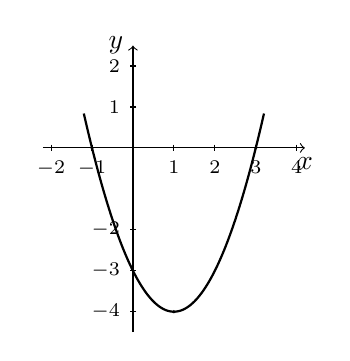
\begin{tikzpicture}[scale=0.52]
    \draw[->] (-2.2,0) -- (4.2,0) node[below] {$x$};
    \draw[->] (0,-4.5) -- (0,2.5) node[left] {$y$};
    \foreach \x in {-2,-1,1,2,3,4}
      \draw (\x,0.08)--(\x,-0.08) node[below] {\scriptsize $\x$};
    \foreach \y in {-4,-3,-2,1,2}
      \draw (0.08,\y)--(-0.08,\y) node[left] {\scriptsize $\y$};
    \draw[smooth, samples=200, domain=-1.2:3.2, thick] plot (\x, {(\x-1)*(\x-1)-4});
    \fill (-1,0) circle (1.2pt);
    \fill (3,0) circle (1.2pt);
    \fill (1,-4) circle (1.2pt);
\end{tikzpicture}
